%%%%%%%%%%%%%%%%%%%%%%%%%%%%%%%%%%%%%%%%%%%%%%%%%%%%%%%%%%%
\subsection{Statistical model design and testing}
%%%%%%%%%%%%%%%%%%%%%%%%%%%%%%%%%%%%%%%%%%%%%%%%%%%%%%%%%%%
%
%
\begin{frame}[t, negative]
	\subsectionpage
\end{frame}
%
%
\begin{lhframe}[rhgraphic={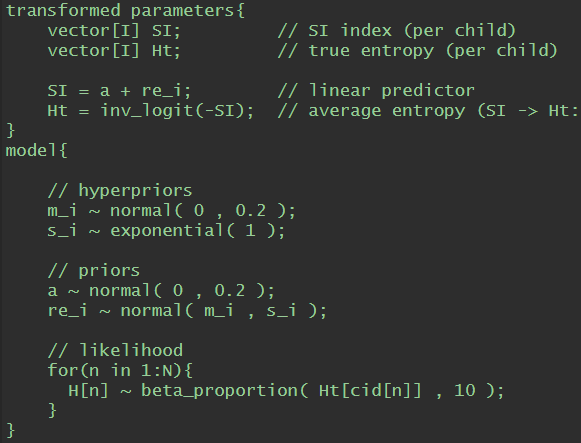
\includegraphics[scale=0.60]{model_design1.png}}]
	{Model design\footnote{Following \citet{Fogarty_et_al_2022}}}
	
	Purpose:
	%
	\begin{itemize}
		%
		\item to have reliable procedures,
		\item to maintain a clear documentation,
		\item to have a sound analysis
		%
	\end{itemize}
	% 
\end{lhframe}
%
%
\begin{lhframe}[rhgraphic={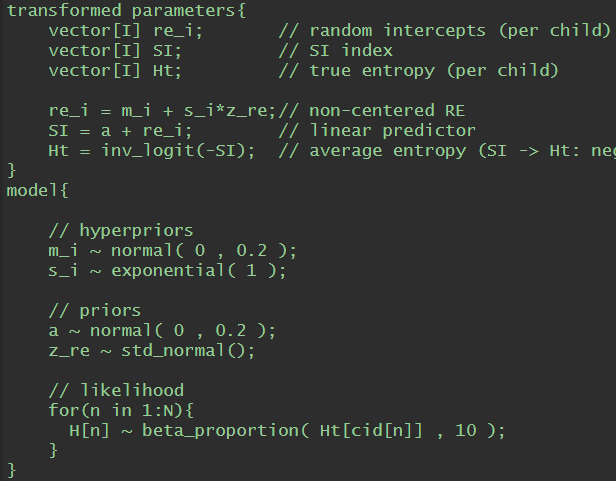
\includegraphics[scale=0.59]{model_design2.png}}]
	{Model design}
	
	Procedure:
	%
	\begin{itemize}
		%
		\item step by step, instantiating one difficulty at the time
		\item Try the centered and non-centered versions
		%
	\end{itemize}
	%
\end{lhframe}
%
%
\begin{lhframe}[rhgraphic={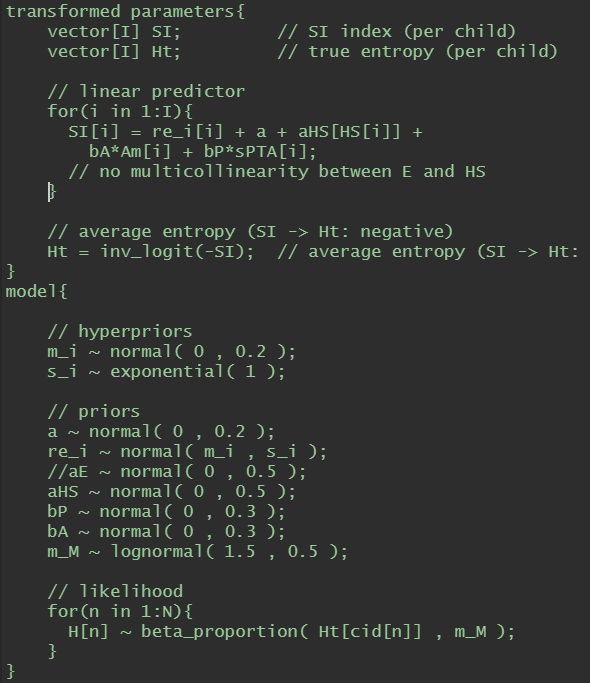
\includegraphics[scale=0.59]{model_design3.png}}]
	{Model design}
	
	In total $5$ random effects models (from $5$ synthetic data types) were tested: 
	%
	\begin{itemize}
		%
		\item only intercept, $M=10$ (centered, non-centered), 
		%
		\item multivariate regression, $M=10$ (centered, non-centered),
		%
		\item multivariate regression, $M$ per individual (centered, non-centered),
		%
		\item no known process (centered, non-centered),
		%
		\item multivariate regression with interaction, $M$ per individual (centered, non-centered),
		%
	\end{itemize}
	%
\end{lhframe}
%
%
\begin{lhframe}[rhgraphic={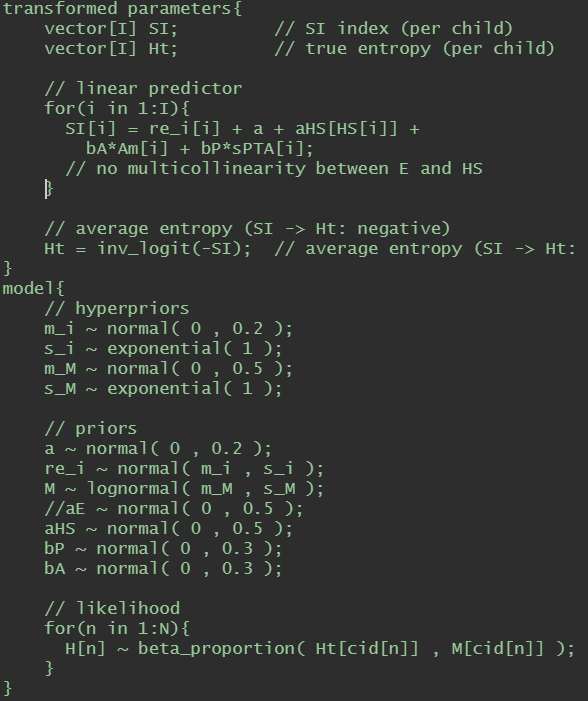
\includegraphics[scale=0.55]{model_design5.png}}]
	{Model design}
	
	Procedure:
	%
	\begin{itemize}
		%
		\item notice we used the hypothesis and (some) probabilistic assumptions defined in section \textcolor{blue}{Estimand and process model}
		%
		\item is like running section \textcolor{blue}{Synthetic data generation} backwards
		%
	\end{itemize}
	%
\end{lhframe}
%
%
\begin{frame}
	{Prior predictive simulation}
	%
	\begin{columns}
		%
		\begin{column}{0.5\textwidth}
			%
			Priors and hyper-priors
			%
			\begin{itemize}
				%
				\item In the \textcolor{blue}{probabilistic (causal) model} there were no priors for our parameters,
				%
				\item To decide our priors we follow \citet{McElreath_2020}: \\ \textcolor{blue}{``priors are part of the assumptions, and should be inspected as such"},
				%
				\item We will evaluate the implications of our priors on the outcome scale. \\
				We have \textcolor{blue}{three outcomes scales}: \\
				$SI_{i}$, $H^{T}_{i}$, and $H^{O}_{ik}$
				%
			\end{itemize}
			%
		\end{column}
		%
		\begin{column}{0.5\textwidth}  
			%
			\begin{equ}
				%
				\begin{aligned} 
					%
					\text{Priors}\\
					a_{i} & \sim \; Normal( \mu_{a}, \sigma_{a}) \\
					M_{i} & \sim \; LogNormal( \mu_{M}, \sigma_{M}) \\
					\alpha & \sim \; Normal( 0, 0.2) \\
					\alpha_{HS[i]} & \sim \; Normal( 0, 0.5) \\
					\alpha_{E[i]} & \sim \; Normal( 0, 0.5) \\ 
					\beta_{A, HS[i]} & \sim \; Normal( 0, 0.3) \\
					\beta_{P} & \sim \; Normal( 0, 0.3) \\
					%
					\text{Hyper-priors} \\
					\mu_{a} & \sim \; Normal( 0, 0.2) \\
					\sigma_{a} & \sim \; Exp(1) \\
					\mu_{M} & \sim \; Normal( 0, 0.5) \\
					\sigma_{M} & \sim \; Exp(1) \\
					%
				\end{aligned}
				%
			\end{equ}
			%
		\end{column}
		%
	\end{columns}
	%
\end{frame}
%
%
\begin{lhframe}[rhgraphic={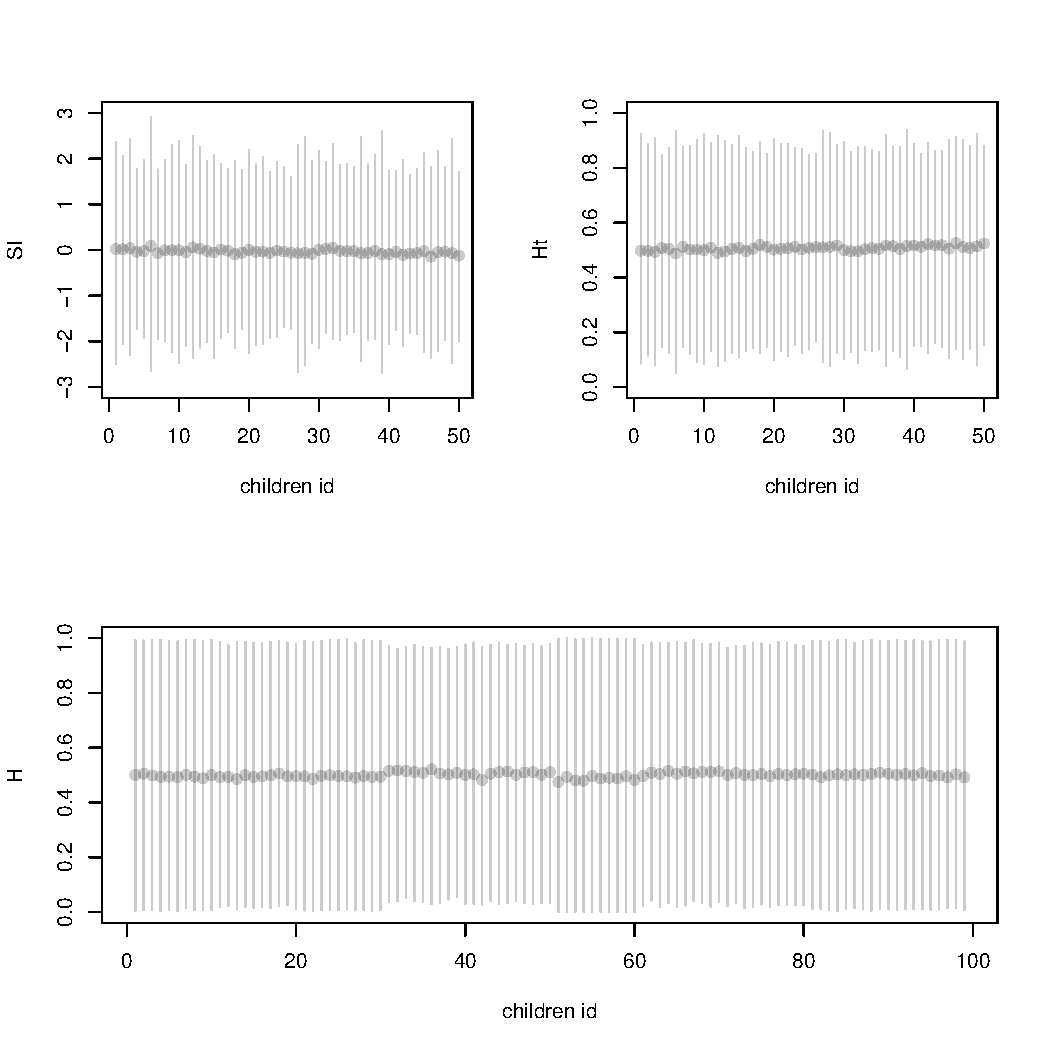
\includegraphics[scale=0.45]{prior_predictive.pdf}}]
	{Prior predictive simulation}
	
	What our priors imply? \\ \\
	\textcolor{blue}{NO undesired assumption} has crept in:
	\begin{itemize}
		%
		\item the $SI_{i}$ scale,
		\item the $H^{T}_{i}$ scale,
		\item the $H^{O}_{ik}$ scale
		%
	\end{itemize}
	
	i.e. the \alert{full space} of the scales \alert{can be reached} by the parameters
	%
\end{lhframe}
%
%
\begin{frame}
	{Parameter recovery}
	%
\end{frame}
%
%
\begin{frame}
	{Posterior predictive}
	%
\end{frame}
%
%
\begin{frame}
	{Power}
	%
\end{frame}
%
%
